\documentclass[tikz,border=4pt]{standalone}
\usepackage[T1]{fontenc}
\usepackage{lmodern,amsmath,mathrsfs}
\usepackage{pgfplots}
\pgfplotsset{compat=1.18}
\definecolor{blue}{HTML}{0072B2}
\definecolor{orange}{HTML}{D55E00}
\definecolor{green}{HTML}{009E73}
\definecolor{purple}{HTML}{CC79A7}
\newcommand{\diamondbackground}{%
 \foreach \c in {-8,-4,-2,-1,-.5,0,.5,1,2,4,8}{
  \draw[gray!24,line width=.18pt] plot[domain=-89.8:89.8,samples=121,variable=\r]
  ({(atan(\c+tan(\r))-atan(\c-tan(\r)))/180},{(atan(\c+tan(\r))+atan(\c-tan(\r)))/180});
  \draw[gray!24,line width=.18pt] plot[domain=-89.8:89.8,samples=121,variable=\r]
  ({(atan(tan(\r)+\c)-atan(tan(\r)-\c))/180},{(atan(tan(\r)+\c)+atan(tan(\r)-\c))/180});
 }
 \draw[black,line width=.7pt] (0,-1)--(1,0)--(0,1)--(-1,0)--cycle;
 \node[above,font=\small] at (0,1) {$i^+$};
 \node[below,font=\small] at (0,-1) {$i^-$};
 \node[left,font=\small] at (-1,0) {$i^0_{\mathrm L}$};
 \node[right,font=\small] at (1,0) {$i^0_{\mathrm R}$};
 \node[above,font=\small] at (-.55,.55) {$\mathscr I^+_{\mathrm L}$};
 \node[above,font=\small] at (.55,.55) {$\mathscr I^+_{\mathrm R}$};
 \node[below,font=\small] at (-.55,-.55) {$\mathscr I^-_{\mathrm L}$};
 \node[below,font=\small] at (.55,-.55) {$\mathscr I^-_{\mathrm R}$};
}
\begin{document}
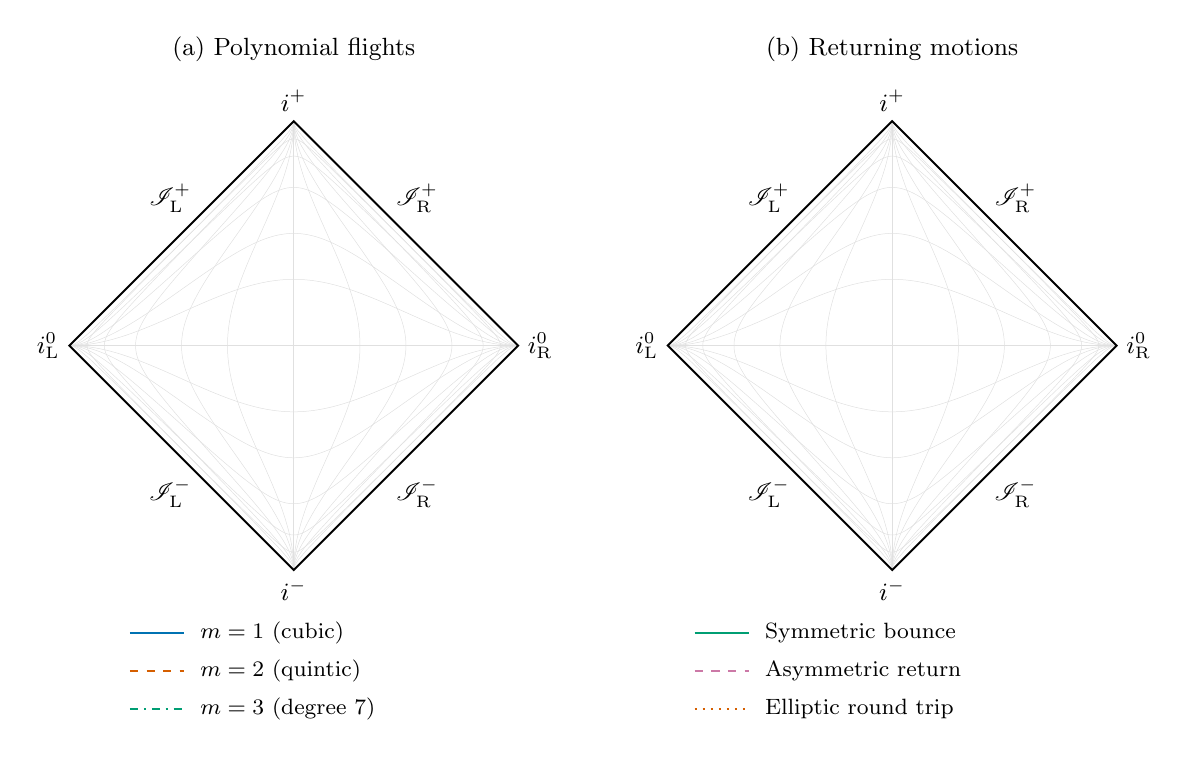
\begin{tikzpicture}[x=2.85cm,y=2.85cm]
\begin{scope}
 \diamondbackground
 \node[font=\small] at (0,1.32) {(a) Polynomial flights};
 \draw[blue,line width=.9pt] plot file {data/penrose_m1.dat};
 \draw[orange,line width=.9pt,dashed] plot file {data/penrose_m2.dat};
 \draw[green,line width=.9pt,dashdotted] plot file {data/penrose_m3.dat};
 \draw[blue,line width=.9pt] (-.73,-1.28)--(-.49,-1.28);
 \node[right,font=\footnotesize] at (-.46,-1.28) {$m=1$ (cubic)};
 \draw[orange,line width=.9pt,dashed] (-.73,-1.45)--(-.49,-1.45);
 \node[right,font=\footnotesize] at (-.46,-1.45) {$m=2$ (quintic)};
 \draw[green,line width=.9pt,dashdotted] (-.73,-1.62)--(-.49,-1.62);
 \node[right,font=\footnotesize] at (-.46,-1.62) {$m=3$ (degree 7)};
\end{scope}
\begin{scope}[xshift=7.6cm]
 \diamondbackground
 \node[font=\small] at (0,1.32) {(b) Returning motions};
 \draw[green,line width=.9pt] plot file {data/penrose_bounce.dat};
 \draw[purple,line width=.9pt,dashed] plot file {data/penrose_asymmetric.dat};
 \draw[orange,line width=.9pt,dotted] plot file {data/penrose_elliptic.dat};
 \draw[green,line width=.9pt] (-.88,-1.28)--(-.64,-1.28);
 \node[right,font=\footnotesize] at (-.61,-1.28) {Symmetric bounce};
 \draw[purple,line width=.9pt,dashed] (-.88,-1.45)--(-.64,-1.45);
 \node[right,font=\footnotesize] at (-.61,-1.45) {Asymmetric return};
 \draw[orange,line width=.9pt,dotted] (-.88,-1.62)--(-.64,-1.62);
 \node[right,font=\footnotesize] at (-.61,-1.62) {Elliptic round trip};
\end{scope}
\end{tikzpicture}
\end{document}

